\chapter{Realization of Concepts}\label{realization}
Based on the concepts presented in the preceding chapter, this chapter
describes the implementation process of the newly created tools and services.
Problems and details specific for the implementation part such as complexity
analysis or architectural features are illustrated. The usage of these
implemented services and tools in the environment of the \ac{SEG} is
additionally focused.
\section{ProfileMatcher}\label{realization:profilematcher}
For supporting the matching of \ac{UML} profiles in SiDiff a new service
has been introduced as part of this Master's Thesis. As shown in
figure~\ref{profilematcher} the matcher itself is executed after all other
SiDiff matching services. The implementation itself is based on the Eclipse
plugin architecture, as the whole \ac{SEG} tool pipeline is evolved around this
ecosystem.

 \begin{figure}[h!]
\begin{center}
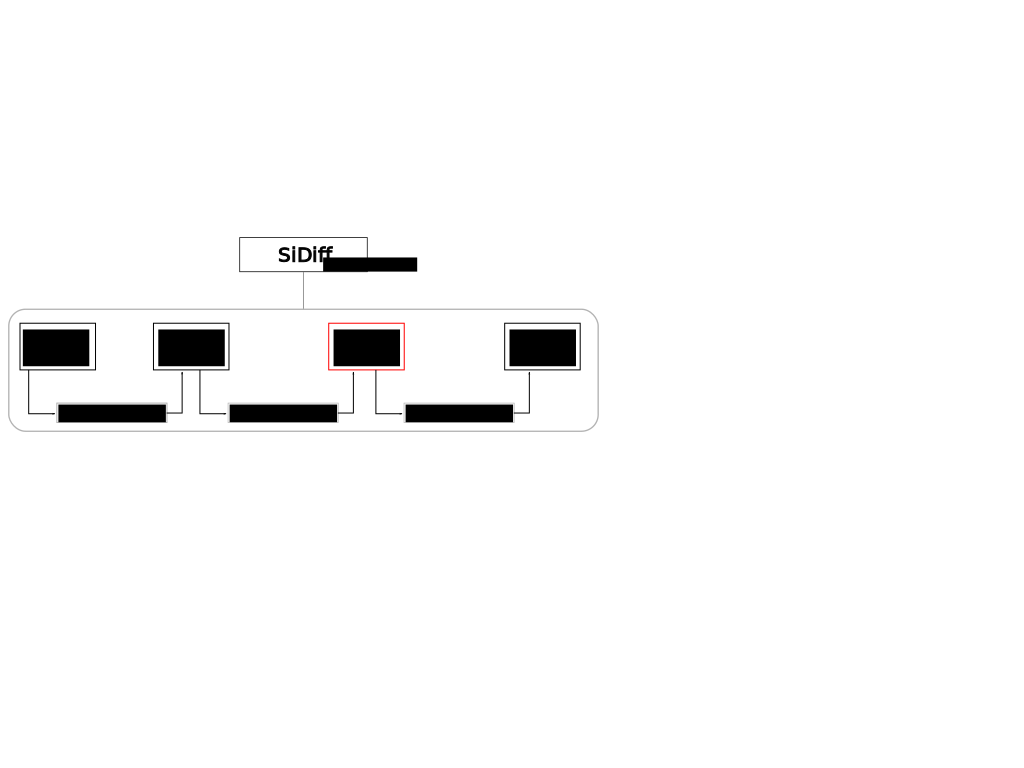
\includegraphics[scale=0.6]{profilematcher}\\
\end{center}
\caption{ProfileMatcher tool integration overview}
\label{profilematcher}
\end{figure}
\newpage

To integrate this service into tools using SiDiff, only a minimal change of code
has to be done by the tool engineer. Complying to the SiDiff service
architecture, the \textit{ProfileMatcher} can be integrated easily:
As described in section~\ref{Integration:sidiff} does the \textit{ProfileMatcher} rely on
computed correspondences, therefore the SiDiff \textit{CorrespondenceService} is
crucial for this matcher to work. Assuming this service has been registered
and is available for usage all needed lines of code to integrate and execute the
new matcher afterwards are depicted in listing~\ref{profilematcher_integration}.
 \lstset{ language=Java,
    caption={ProfileMatcher service integration},
    label=profilematcher_integration
    }
    \begin{lstlisting}
    //Define configuration file
    private final static String profileFileName = "uml.profiles.xml";
   
    //Configure ProfileMatcher according to configuration
    ServiceHelper.configureInstance(context, ProfilesMatchingService.class,
				UML_URI, null, profileFileName);
				
    //Register SiDiff service
  	ServiceContext.putService(ServiceHelper.getService(Activator.context,
  	ProfilesMatchingService.class, documentType, ServiceHelper.DEFAULT));
					
 	 //Execute ProfileMatcher service					
	 ServiceContext.getService(ProfilesMatchingService.class).match();\end{lstlisting}

As explained in detail in section~\ref{Integration:sidiff} one advantage of the
implemented matcher is the reduced effort needed for the configuration of
the service. The configuration syntax is based on other SiDiff
configurations like the one of the similarity matcher. The configuration of profiles is done like
depicted in listing~\ref{profilematcher_configuration}.

\lstset{
    language=XML,    
    morekeywords={name,encoding, base Package, stereo Package},
    caption={ProfileMatcher configuration example},
    label=profilematcher_configuration
    }
\lstinputlisting{attachments/org.sidiff.sysml.core.profileconfig.xml}

One configuration file can hold multiple \ac{UML} profiles such as the one
defined in line 4. Each profile can be configured in detail if necessary by
creating a white list of profiling elements, whereas the absence of such list
will use all existing profiling elements contained in the given \ac{UML}
profile, like done in listing~\ref{profilematcher_configuration}. The
matcher will iterate through all given profiles and match their white list
elements accordingly to their meta model automatically, therefore no additional
configuration is needed. The execution of the profile matching service will
engage the following actions for each configured profile:
\begin{itemize}
  \item Read the given configuration file and analyze the corresponding meta
  model according to this configuration.
  \item Save all profiling elements, their corresponding base element and the
  relationship reference between them in a map. 
  \item Build a map between both the profiling elements as well as the base
  elements.
  \item Iterate through all correspondences and search for base elements.
  \item Add a new correspondence to the respective profiling element if such
  base element is found in the correspondence as well as the built map.
\end{itemize}
\section{UUIDFixer}\label{realization:uuidfixer}
As the ProfileMatcher described in the preceding section, the \ac{UUID}Fixer is
implemented using the Eclipse plugin architecture and makes use of the SiDiff
service environment. 

 \begin{figure}[h!]
\begin{center}
\includegraphics[scale=0.6]{uuidfixer}\\
\end{center}
\caption{\ac{UUID}Fixer tool integration overview}
\label{uuidfixer}
\end{figure}

The integration part of this service is even more easily to be done, as there is
no need for any configuration at all(listing~\ref{uuidfixer_integration}). As
the ProfileMatcher, the \ac{UUID}Fixer makes use of the
\textit{CorrespondenceService} and is therefore most effective if executed as
last SiDiff service, as at this time more correspondences could be available.

 \lstset{ language=Java,
    caption={\ac{UUID}Fixer service integration},
    label=uuidfixer_integration
    }
    \begin{lstlisting}				
    //Register SiDiff service
  	ServiceContext.putService(ServiceHelper.getService(Activator.context,
  	IDFixerService.class, null, null));
					
 	 //Execute UUIDFixer service					
	 ServiceContext.getService(IDFixerService.class).fixIDs();\end{lstlisting}

The id fixing service algorithm can be divided into the following parts for each
model element $A$:
\begin{enumerate}
  \item Get corresponding element $B$ of current element $A$, if any.
  \item Compare the \ac{UUID}s of both elements $A$ and $B$ with each other.
  \item If they are not equal, replace the identifier of $B$ with the one of
  $A$.
\end{enumerate} 
As already denoted earlier, the replacement of the \ac{UUID} is done
in $B$ as it is the \textit{newer} model which is the one to fix. This
convention originates from the repository domain, as the fixing in $A$ would destroy
possible correspondences between $A$ and earlier revisions.
\section{ProfileApplicator}\label{realization:profileapplicator}
\begin{figure}[h!]
\begin{center}
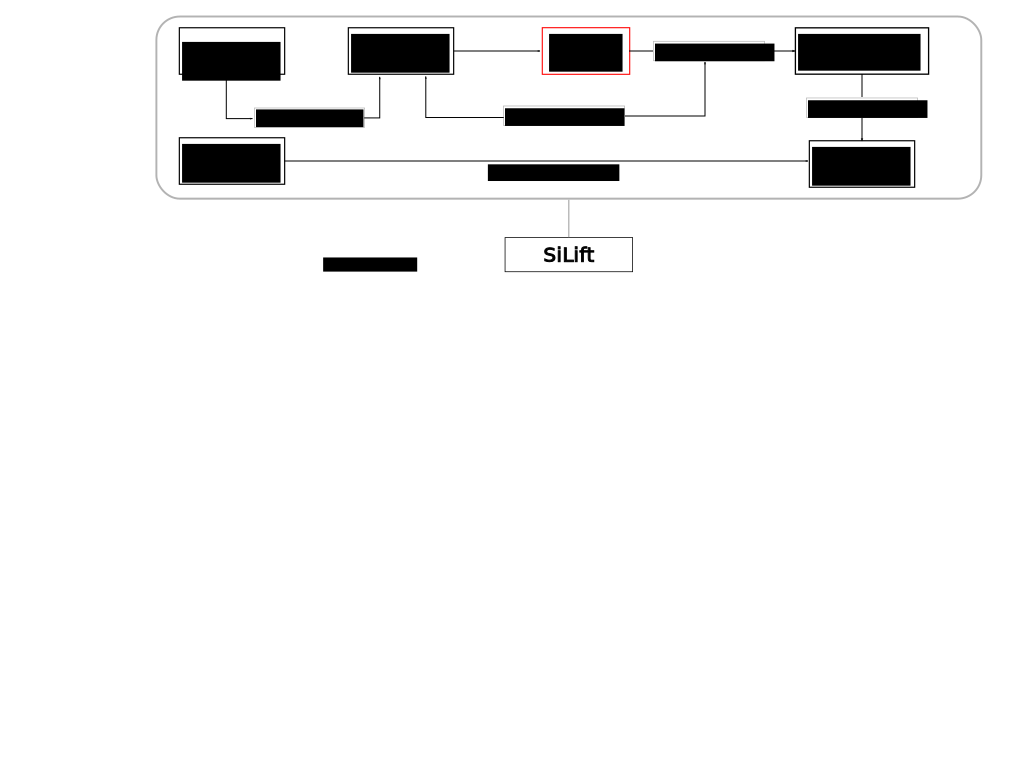
\includegraphics[scale=0.5]{profileapplicator}\\
\end{center}
\caption{ProfileApplicator tool integration overview}
\label{profileapplicator}
\end{figure}
Contrary to the previous services the \textit{ProfileApplicator} has been
implemented as an OSGi application, as it is used as standalone tool in the SiLift context.
The software architecture internally is similar to the one of \ac{SERGe}, as
they are used in the same manner and often even consecutively. As \ac{SERGe}
itself, the \textit{ProfileApplicator} has its own configuration for a detailed adaption
by the tool engineer, whereas the semantics of the configuration shall be
explained in detail. Considering the profile settings depicted in
listing~\ref{profileapplicator_profilesettings}, the following configuration
possibilities are available:

\begin{itemize}
  \item \textbf{Name} \\
  		This defines a human readable name for this \ac{UML} profile, which serves
  		as debug output and more understandable output possibilities in general.
  \item \textbf{BaseTypeInstances} \\
  		As the name suggests, does this option toggle the possibility of instances 
  		containing only the base element. As example the \textit{Class} /
  		\textit{Block} relationship seems appropriate: If the option is set to
  		\textit{false}, there shall be no \textit{Class} element without a profiling element \textit{Block}, whereas if set
  		to \textit{true} the result will be two edit rules, one containing only the
  		\textit{Class} element, the other containing both.
  \item \textbf{BaseTypeInheritance} \\
  		This option defines whether the ProfileApplicator should only take the
  		direct relationship and its corresponding base element of a give profiling
  		elements into consideration. Using \ac{SysML} as profile, the defined
  		element \textit{RequirementRelated} is added to every \textit{NamedElement}.
  		Disabling BaseTypeInheritance would result in no additional rule, as
  		\textit{NamedElement} is abstract and therefore cannot be instantiated. Enabling
  		would result in multiple result rules, as many concrete elements are of the
  		type \textit{NamedElement}, for example the \textit{Class} element.
\end{itemize}
\lstset{
    language=XML,    
    morekeywords={name,encoding,allow,nsUri,apply, basePackage, stereoPackage},
    caption={ProfileSettings configuration example},
    label=profileapplicator_profilesettings}
\lstinputlisting[firstline=4,lastline=8]{attachments/org.sidiff.profileapplicator.sysmlConfig.xml}
For additional adaption possibilities, the configuration part presented in
listing~\ref{profileapplicator_transformations} is available: The tool engineer
can decide which \ac{HOT} will be used by the \textit{ProfileApplicator},
declaring which type of Henshin nodes will taken into consideration for transformation.
\newpage
 \lstset{
    language=XML,    
    morekeywords={name,encoding,allow,nsUri,apply, basePackage, stereoPackage},
    caption={Transformations configuration example},
    label=profileapplicator_transformations}
\lstinputlisting[firstline=15,lastline=19]{attachments/org.sidiff.profileapplicator.sysmlConfig.xml}

Like the white list implemented in the profile matching service, does the
\textit{ProfileApplicator} also support this functionality. If none profiling element is defined, all
elements of the given \ac{UML} profile will be used. If on the other hand at
least one has been added, only these are used for transformation. This
configuration style has been used in \ac{SERGe} as well and therefore has been
implemented this way.

The execution of the tool needs additionally to the configuration
explained above two parameters, which can be defined by the user via an input
dialog presented by an OSGi execution configuration:
\begin{itemize}
  \item Folder of base type Henshin edit rules to transform (e.g. containing
  \ac{UML} edit rules).
  \item Target folder for saving the resulting transformed edit rules (e.g.
  \ac{SysML} folder).
\end{itemize}

While implementing the \textit{ProfileApplicator}, various runtime problems have
arisen, which needed a feasible solution. The transformation tool used by the
profile application tool is Henshin, which itself relies on Ecore~\cite{EcoreURL} for
internal model representation. Each \textit{EObject} loaded will register an
\textit{Action Listener}, which is capable of detecting changes concerning this
object.
Using the functionality on default, each \textit{EObject} will contain such listener and
each element referring to this EObject will create a
\textit{CrossReferenceAdapter}. Using large meta models like \ac{UML} will lead
to huge numbers of such adapters and listeners between all elements. This will
lead to an exponential growth while executing the ProfileApplicator, which
therefore will not finish its transformation in finite runtime. The solution is
presented as listing~\ref{listener_example}: All elements contained in an
\textit{EGraph} used by Henshin will be deleted manually, therefore all adapters
and cross references will be removed as well.
\newpage
 \lstset{ language=Java,
    caption={Deleting all EObjects manually},
    label=listener_example
    }
    \begin{lstlisting}
  public void releaseAdapters(EGraph graph) {		
    	for (EObject roots : graph.getRoots()) {
				graph.removeGraph(roots);
			}
	}\end{lstlisting}
	 
The deletion process uses some computation time itself, but the
the final runtime of the tool is constant and therefore ends
in finite runtime. Deleting these objects manually leads to the result shown in
figure~\ref{objectNumberReport} taken while executing the profile application.

 \begin{figure}[h!]
\begin{center}
\includegraphics[scale=0.5]{objectNumberReport}\\
\end{center}
\caption{Objects contained in an EGraph}
\label{objectNumberReport}
\end{figure}

Another runtime problem concerning the used \textit{EGraph} itself has arisen
during development. By default the constructor of such a Henshin EGraph will resolve
all object references of the given input model and will add the referenced
objects additionally to this EGraph. Given a large model like \ac{UML} as
input results in an enormous graph, which must be searched during the execution
of a Henshin rule. Henshin tries to match the preserve nodes as previously
described, whereas the number of nodes has a large impact on runtime. Adding
only the used elements into the EGraph manually instead of using the default
constructor leads to a considerable smaller EGraph and therefore runtime.
The code snippet of this solution is depicted in listing~\ref{egraph_solution}.
This solution reduced the EGraph size from $7463$ to $27$ for example, which
drastically effects the runtime.

 \lstset{ language=Java,
    caption={Manually adding needed elements to an EGraph},
    label=egraph_solution
    }
    \begin{lstlisting}
 	// Create Module EGraph and its children as working copy
	workGraph = new EGraphImpl();
	workGraph.addTree(workResourceSet.getModule(this.sourceFile.getName()));

	// Add all important elements for matching
	workGraph.add(applicator.getStereoPackage());

	// Add Stereotype and its Attributes
	workGraph.add(stereoType.getStereoTypeClass());
	for (EStructuralFeature feature : stereoType.getStereoTypeClass().getEAllStructuralFeatures()) {
		workGraph.add(feature);
	}
	
	//Add Basetype and baseReference
	workGraph.add(baseType);
	workGraph.add(stereoType.getBaseTypeMap().get(baseType));\end{lstlisting}

For further runtime improvement the ProfileApplicator implements the Java
threading technology as using threads in today's multicore environments seems
appropriate. Each profile applicator thread transforms one input Henshin edit
rule, therefore no concurrency problems can arise. Each input edit rule is
defined as work package which needs to be transformed. It is placed in a work pool, whereas each
thread can remove such a package for transformation. As the number of
threads used for computation are configurable via an execution parameter, 
each tool user can adapt this technology to his own needs. Having each thread
computed parallel reduces the runtime by a factor of threads e.g. having 4 threads 
executed on a quadcore processor leads to a runtime reduction by a factor close
to 4.
